\documentclass[11pt,a4paper,USenglish,twocolumn]{article}
\usepackage{unir_paper}


%---------------------------
%título del trabajo y autor
%---------------------------
\title{Machine Learning Tools for Open Cluster Characterization with Gaia DR2 Data}
\author{Carlos David Álvaro Yunta}
\date{24th of January, 2021}


%---------------------------
%marges
%---------------------------
%\usepackage[margin=1.9cm]{geometry}
%---------------------------
%---------------------------
%---------------------------
%---------------------------

\resumen{
The characterization and understanding of \emph{Open Clusters}
allow us to better understand properties and mechanisms about the Universe
such as stellar formation and the kind of regions where these events occur.
They also provide information about stellar processes and the evolution of the galactic disk.

In this paper, we develop a method to characterize open clusters by using
\emph{artificial intelligence} tools, such as clustering by \emph{K-Means}
and clustering based on \emph{Artificial Neural Networks} by implementing
the \emph{Deep Embedded Clustering} model.
We are using \emph{Gaia DR2 database} as data source for testing our models.

The developed method aims to improve current techniques of the state of the art.
We achieve improvements not only in terms of \emph{computational efficiency},
with lower computational requirements, but in \emph{usability},
reducing the number of hyperparameters to obtain a good characterization of the analyzed clusters.

Our method achieves good results,
becoming even better in some cases when the results are compared with current techniques.
}

\palabrasclave{
    characterization,
    data analysis,
    deep embedded clustering,
    gaia,
    machine learning,
    open cluster
}

\begin{document}
\twocolumn[
\begin{@twocolumnfalse}
\maketitle
\end{@twocolumnfalse}
]

%\renewcommand{\listfigurename}{Índice de Ilustraciones}
%\renewcommand{\listtablename}{Índice de Tablas}
%\renewcommand{\contentsname}{Índice de Contenidos}
%\renewcommand{\figurename}{Figura}
%\renewcommand{\tablename}{Tabla}
%\twocolumn


%\frontmatter
%\tableofcontents
%\listoffigures
%\listoftables

\section{INTRODUCTION}

Stellar open clusters (OCs) \cite{janes1982open} are groups of stars
gravitationally bounded originated from a single molecular gas cloud.
They share the same chemical composition and age. Moreover,
they have similar relative positions and proper motion.
Those astronomical objects are relevant to understand the spiral structure,
the dynamics and the chemical evolution of our galaxy.

The study of OCs has been pushed forward thanks to the huge and precise dataset
from the Gaia mission Gaia DR2 available since 2018
\cite{collaboration2016description} and \cite{gaia2018gaia}.
This dataset has helped to review already known open clusters and to find new ones.

Stars that belong to the same OC share relative positions,
inherited from their original gas cloud.
This means that their distances to the Earth are similar for all of them and,
therefore, they have a narrow dispersion in their parallax value.
They also share similar values of proper motion, both in right ascension and declination.
Another property they share is their chemical composition.
Thus, their metallicity must be uniform,
since these stars were born from the same gas cloud and at the same time stage.
However, to take this last property into account, we are faced with the drawback
that this parameter is poorly reported in Gaia DR2 database.

Normally, the characterization process takes into account astrometric features
such as proper motion in right ascension and declination, and parallax.
And photometric features like $E(b-r) / G_{mag}$.
Photometric variables are used for generating the H-R diagram of the OC candidate stars.
This stars should present a sharp profile corresponding to an isochrone curve derived
from a theoretical model.
This model does consider metallicity, mass and brightness of the stars involved.
At the moment, a set of tools have been used for this purpose, as explained later,
but in general, these tools require supervised and parameterized models.
So a previous knowledge of the cluster is necessary or the process must be repeated
iteratively in order to achieve valid results.

Our aim is to build a machine learning model capable of characterizing open
clusters inside a stellar region without previous knowledge of that region.
This model will take advantage of these features to train an Artificial Neural
Network (ANN) that will clusterize all stars within the given region.
One of these groups will be the open cluster that interests us.
With that purpose we have adapted the Unsupervised Deep Embedding for Clustering
Analysis \cite{xie2016unsupervised} to our problem.

This model fulfills one of our main requirements.
It has to be \emph{non-supervised} and \emph{non-parameterized} in order to make easier
the automation process of analyzing a wide range of regions with different topologies.
Another important requirement for our model is that it must be computationally efficient
in order to run in common workstations.
The model has been developed with Python using the Keras framework which takes
advantage of modern GPUs to make its computations.
That increases significantly the computational capacity of our model making possible
to run it on regular workstations with one of those GPUs.

Since the aim of this work is not to find new OCs but to improve the characterization
of the already known ones, we have taken the approach of analyzing known regions.
These regions have been taken from the OpenClust catalogue \cite{dias2002new}
(see Figure \ref{fig:openclust_catalogue}) and downloaded from Gaia DR2 database
increasing the radius of each region by a factor $1.5$.

\begin{figure}
    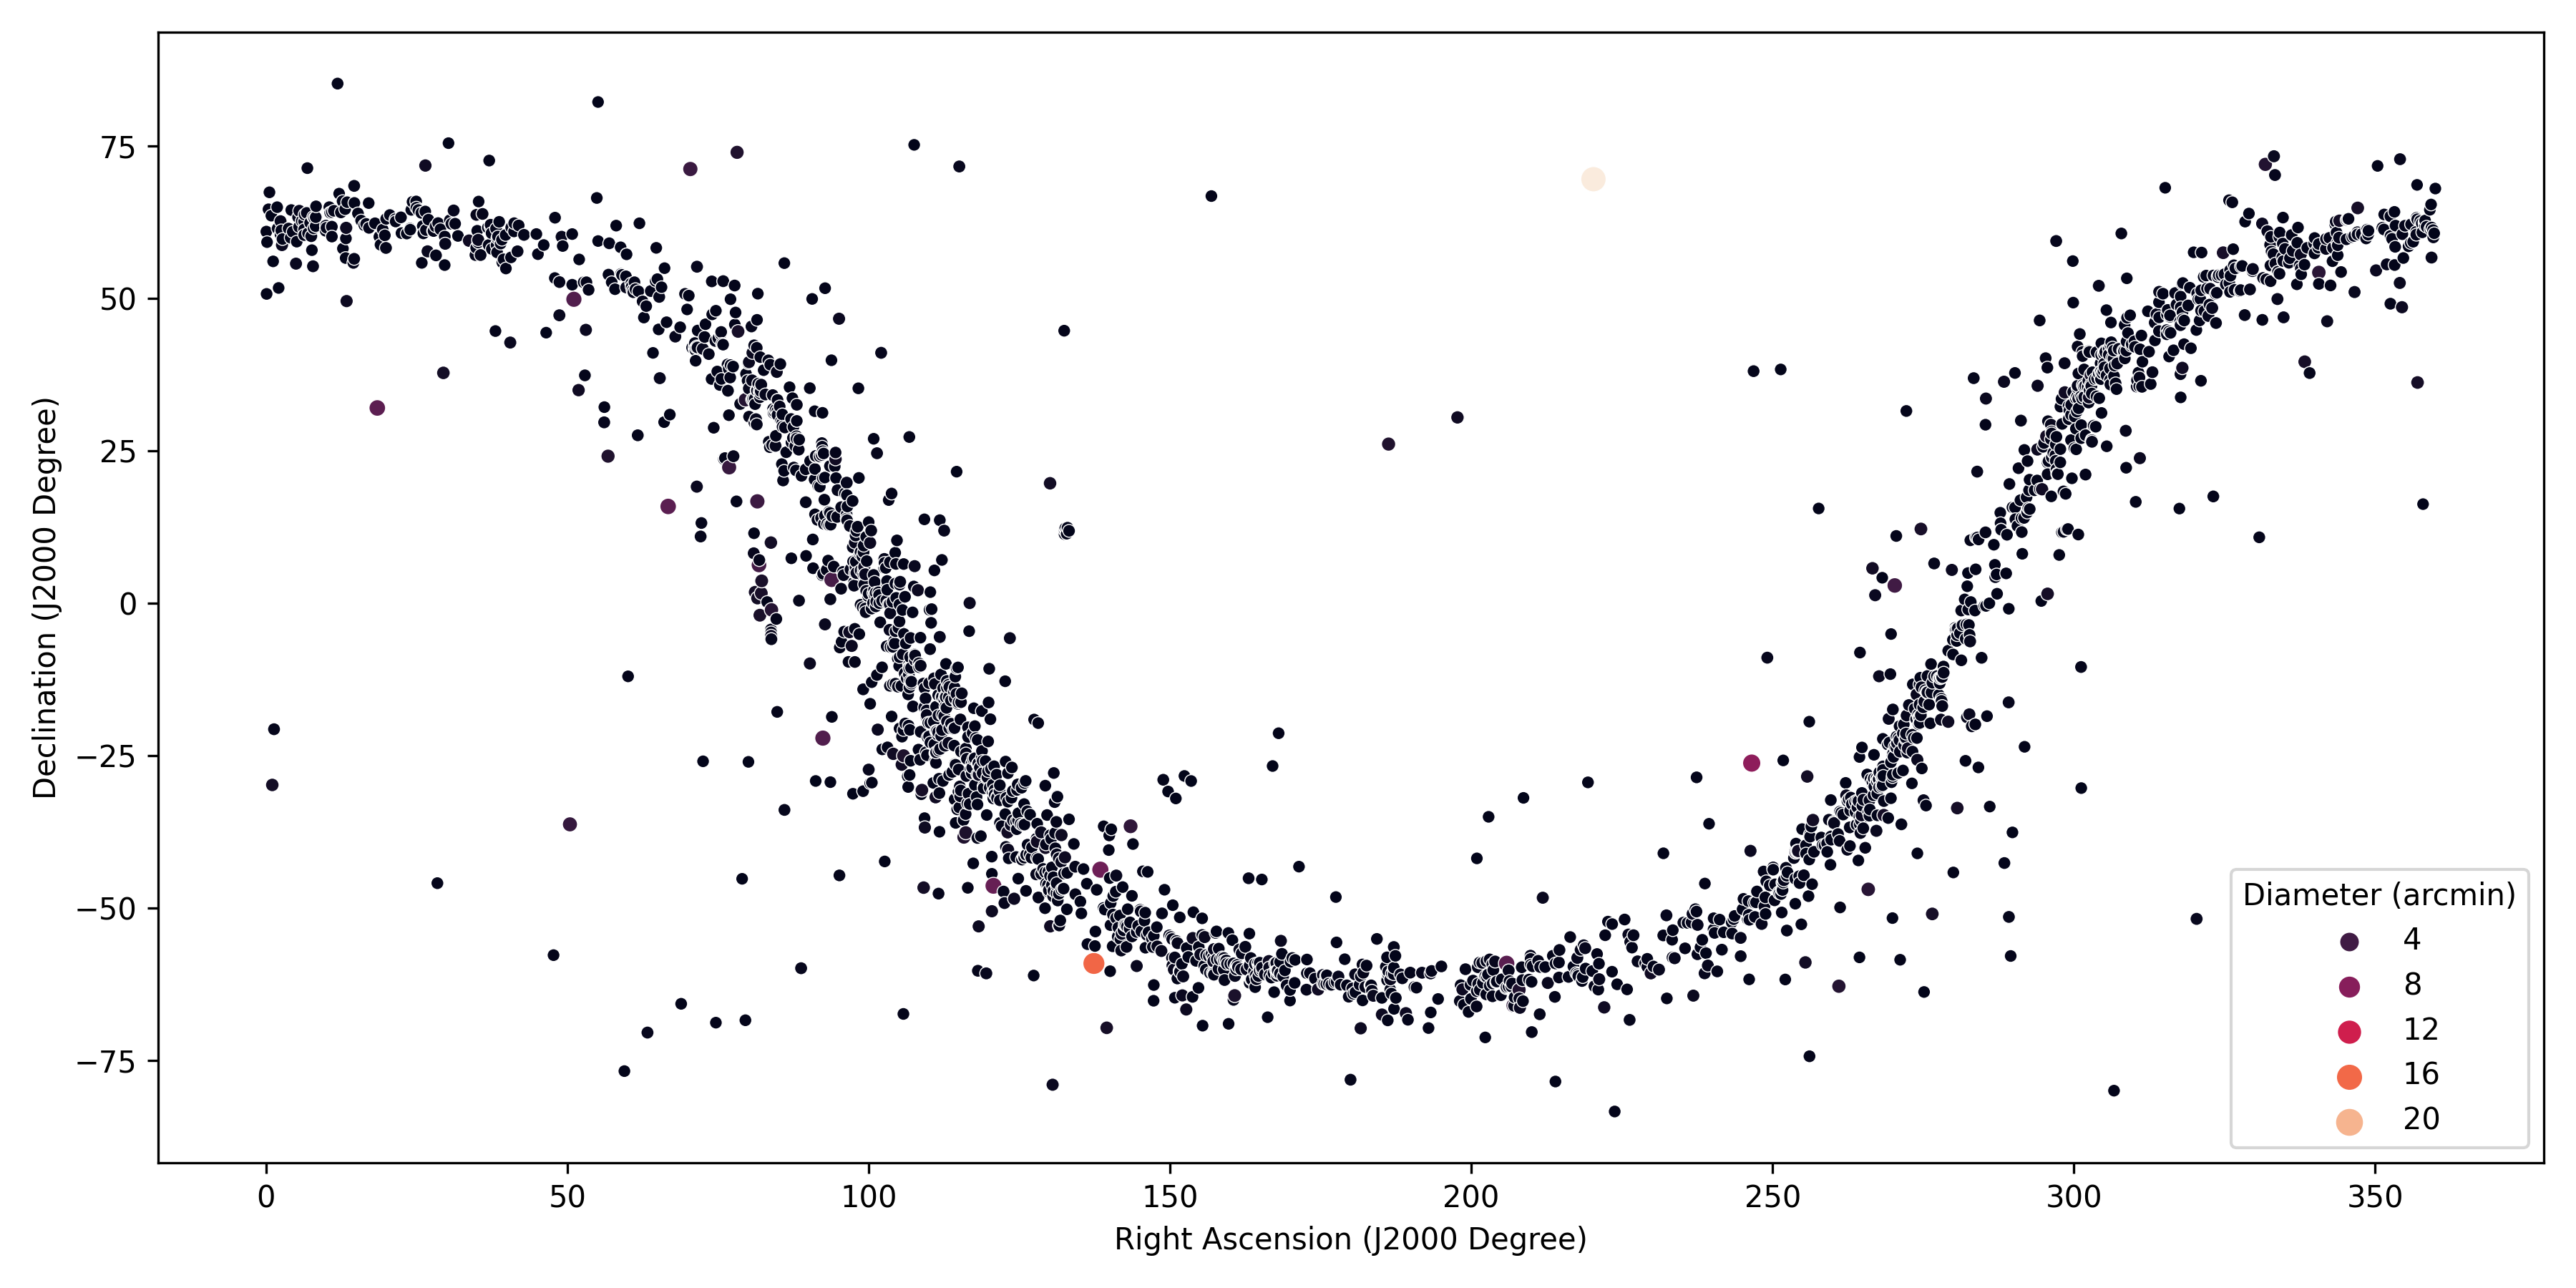
\includegraphics[width=\columnwidth]{../figures/openclust_catalogue.png}
    \caption{OpenClust Catalogue Distribution}
    \label{fig:openclust_catalogue}
\end{figure}

Finally, we have compared the results obtained with the model we purposed with another
method that involves tools from the Virtual Observatory such as Clusterix \cite{balaguer2020clusterix}.

As shown in Section \ref{sec:results}, the results obtained are promising.
Although some improvements must be done in order to consider it as valid tool
that could be part of the standard set of tools for open clusters characterization.

\section{STATE OF THE ART}

Estudio a fondo el dominio de aplicación, citando numerosas referencias.
Debe aportar un buen resumen del conocimiento que ya existe en el campo de los problemas habituales identificados.
\section{AIMS AND METHOD}

Objetivo general, objetivos específicos y metodología de trabajo aplicada.

\section{CONTRIBUTION}

\section{RESULTS}
\label{sec:results}

\subsection{Evaluación 1}

\subsection{Evaluación 2 }
En la Tabla \ref{tab_1}
\begin{table}\label{tab_1}
\caption{Unidades de las propiedades magnéticas:}

\begin{tabular}{ccc}\hline\hline
Símbolo & Cantidad & Conversión\\
\hline
$\Phi$ & flujo magnético & $1$Mx $\rightarrow 10^{-8}V\cdot s$\\
... &...&...\\
\hline\hline
\end{tabular}
\end{table}

\section{RESULTS DISCUSSION}

Tras la presentación objetiva de los resultados, querrás aportar una discusión de los mismos.

\section{CONCLUSIONS}

Resumen de las contribuciones del trabajo, en el que relaciones las contribuciones y los resultados obtenidos con los objetivos que habías planteado para el trabajo, discutiendo hasta qué punto has conseguido resolver los objetivos planteados.
Finalmente, hablar de líneas de trabajo futuro que podrían aportar valor añadido al TFM realizado. La sección debería señalar las perspectivas de futuro que abre el trabajo desarrollado para el campo de estudio definido. En el fondo, debes justificar de qué modo puede emplearse la aportación que has desarrollado y en qué campos.

\appendix
\section{APPENDIX}
Apéndices, en caso de ser necesario.

\renewcommand{\refname}{REFERENCES}
\bibliographystyle{unsrt}
\bibliography{references}

\end{document}
